\documentclass{beamer}
\usepackage{bcprules}
\usepackage{presentation}
\begin{document}
\title{Three Perspectives on Change}
\author{Daniel Wagner}
\date{February 7, 2011}

\maketitle

\begin{frame}
    \frametitle{Diff Format}
    \tiny\texttt{
        \color{green!55!black} \\
        --- presentation.tex        2011-01-27 00:23:42 UTC (rev 443) \\
        +++ presentation.tex        2011-01-27 01:16:46 UTC (rev 444) \\[4ex]
        \color{yellow!80!black}
        $@@$ -1,4 +1,4 $@@$ \\
        \color{orange}
        -\textbackslash documentclass\{beamer\} \\
        \color{blue}
        +\textbackslash documentclass[14pt]\{beamer\} \\
        \color{gray}
        \ \textbackslash usepackage\{array\} \\
        \ \textbackslash usepackage\{graphicx\} \\
        \ \textbackslash usepackage\{tikz\} \\
        \color{yellow!80!black}
        $@@$ -25,8 +25,8 $@@$ \\
        \color{gray}
        \ \quad\textbackslash vpause \\[3ex]
        \ \quad\textbackslash begin\{itemize\} \\
        \color{orange}
        -\quad\quad\textbackslash item At home: tree-structured hierarchical file-system \\
        -\quad\quad\textbackslash item On the web: flat-list gallery of pictures and tags \\
        \color{blue}
        +\quad\quad\textbackslash item At home: tree-structured file-system \\
        +\quad\quad\textbackslash item On the web: flat-list picture gallery with tags \\
        \color{gray}
        \ \quad\textbackslash end\{itemize\} \\
        \ \textbackslash end\{frame\} \\
    }
\end{frame}

\newcommand{\ccommon}{\color{orange}common\color{black}}
\newcommand{\ctools}{\color{yellow!80!black}tools\color{black}}
\begin{frame}
    \frametitle{Git File Tracking}
    \texttt{\\
        \color{gray}
        On branch
        \color{black}
        master
        \color{gray} \\
        Changes to be committed: \\
        \quad(use "git reset HEAD <file>\ldots" to unstage) \\[4ex]
        \quad\quad\begin{tabular}{ll}
            \alert{modified}:  & \ccommon/filetype.h \\
            \alert{renamed}:   & \ctools/grep.h -> \ccommon/grep.h \\
            \alert{new file}:  & \ccommon/wc.h \\
            \alert{deleted}:   & \ctools/wc.h
        \end{tabular}
    }
\end{frame}

\newcommand{\csuppliers}{\color{orange}suppliers\color{black}\xspace}
\newcommand{\ccustomers}{\color{blue}customers\color{black}\xspace}
\begin{frame}
    \frametitle{SQL}
    \small
    \texttt{
        \\
        \alert{update} \csuppliers \alert{set} supplier\_name = \\
        \quad (\alert{select} \ccustomers.name \\
        \quad\ \alert{from} \ \ \ccustomers \\
        \quad\ \alert{where} \ \ccustomers.customer\_id = \csuppliers.supplier\_id) \\[4ex]
        \quad\alert{where exists} \\
        \quad\quad(\alert{select} \ccustomers.name \\
        \quad\quad\ \alert{from} \ \ \ccustomers \\
        \quad\quad\ \alert{where} \ \ccustomers.customer\_id = \csuppliers.supplier\_id);
    }
\end{frame}

\newcommand{\cxsl}[1]{\alert{xsl:#1}}
\newcommand{\cattr}[2]{\color{orange}#1\color{black}=\color{gray}"#2"\color{black}}
\begin{frame}
    \frametitle{XSLT}
    \texttt{
        \\
        <?xml \cattr{version}{1.0}?> \\
        <\cxsl{stylesheet} \cattr{version}{1.0} \\
        \quad\quad \cattr{xmlns:xsl}{http://www.w3.org/1999/XSL/Transform}> \\
        \quad<\cxsl{template} \cattr{match}{/}> \\
        \quad\quad<\cxsl{for-each} \cattr{select}{catalog/cd}> \\
        \quad\quad\quad\color{blue}<tr> \\
        \quad\quad\quad\quad<td>\color{black}<\cxsl{value-of} \cattr{select}{title}/>\color{blue}</td> \\
        \quad\quad\quad\quad<td>\color{black}<\cxsl{value-of} \cattr{select}{artist}/>\color{blue}</td> \\
        \quad\quad\quad</tr>\color{black} \\
        \quad\quad</\cxsl{for-each}> \\
        \quad</\cxsl{template}> \\
        </\cxsl{stylesheet}>
    }
\end{frame}

\begin{frame}
    \frametitle{Emacs Lisp}
    \texttt{
        \\
        (save-excursion \\
        \quad(if (and (boundp 'slime-repl-input-start-mark) \\
        \quad\quad\quad slime-repl-input-start-mark) \\
        \quad\quad(slime-repl-beginning-of-defun) \\
        \quad\quad(beginning-of-defun)) \\
        \quad(\color{orange}paredit-wrap-sexp\color{black}\ n) \\
        \quad(\color{orange}insert \color{gray}"eval-when (:compile-toplevel "\color{black}) \\
        \quad(\color{orange}insert \color{gray}":load-toplevel :execute)\textbackslash n"\color{black}) \\
        \quad(\color{orange}slime-reindent-defun\color{black})) \\
    }
\end{frame}

\section{Perspective 1: Formalizing the Behavior of Revision Control Systems}

\begin{frame}
    \frametitle{Background}
    \begin{itemize}
        \item \emph{Revision control system} -- tools for tracking and
            sharing changes to a codebase
        \item \emph{Working copy} -- the current state of the codebase
        \item \emph{Patch} -- a change to the codebase
        \item \emph{Revision history} -- information about previous (or
            future) states of the codebase and patches
        \item \emph{Repository} -- one of many disjoint locations that track
            a revision history
    \end{itemize}
\end{frame}

\begin{frame}
    \frametitle{Model}
    Keep the model as simple as possible:
    \begin{itemize}
        \item A \emph{working copy} is a set of primitive atoms.
        \item Recover structure via \emph{invariants}.
    \end{itemize}
\end{frame}

\begin{frame}
    \frametitle{Traditional Trees}
    Traditional presentation of a labeled tree:
    \begin{itemize}
        \item Tuple $(N,E,C,f)$
        \item $N$ the set of nodes
        \item $E$ the set of edges, with no cycles
        \item $C$ a set of possible contents
        \item $f : N \to C$ a labeling function
    \end{itemize}
    How can we recover this structure in a working copy?
\end{frame}

\newcommand{\fcontains}{\ \mathbf{contains}\ }
\begin{frame}
    \frametitle{Single-Set Trees}
    An isomorphic presentation:
    \begin{itemize}
        \item Two kinds of atomic facts
            \begin{itemize}
                \item $\ell_p \to \ell_c$
                \item $\ell \fcontains c$
            \end{itemize}
        \item Set $d$ contains facts
        \item Prove properties about $d$ to show that
            \begin{itemize}
                \item $\ell_p \to \ell_c$ facts encode edges and are tree-like
                \item $\ell \fcontains c$ facts are functional and encode the nodes
            \end{itemize}
    \end{itemize}
\end{frame}

\begin{frame}
    \frametitle{On Flexibility}
    \begin{itemize}
        \item A single set is sufficient
        \item For other structures: vary the atoms and invariants
        \item Atom-agnostic definitions apply to any such structure
    \end{itemize}
\end{frame}

\newcommand{\patch}[1]{\mathrel{\tikz\draw[|->]
    node (T) {$#1$}
    (T.south) node {} % for alignment
    (T.south west) -- (T.south east)
    ;}}
\newcommand{\dpatch}{\patch\ }
\begin{frame}
    \frametitle{Model}
    A \emph{patch} is a triple $S \patch E T$:
    \begin{itemize}
        \item Source set $S$ of facts to remove
        \item Target set $T$ of facts to add
        \item Environment set $E$ with $S \cup T \subset E$
    \end{itemize}

    \vpause

    Abbreviate $S \patch{S \cup T} T$ as $S \dpatch T$.
\end{frame}

\tikzstyle{patched}=[color=green!75!black,thick,dashed]
\begin{frame}
    \frametitle{Example}
    When the labeling function is bijective, write $\{A \to B\}$ for
    \[\{\ell_p \to \ell_c,\ell_p \fcontains A,\ell_c \fcontains B\}\]

    \begin{tikzcenter}
        \node (A) {A}
            child { node (B) {B} }
            child { node (C) {C} }
            child[patched] { node (D) {D} }
            ;
    \end{tikzcenter}
    \[d = \{A \to B, A \to C\}\]

    \vpause

    \[\emptyset \dpatch \{A \to D\}\]
\end{frame}

\begin{frame}
    \frametitle{Example: Bad}
    \begin{tikzcenter}
        \node(A) {A}
            child { node (B) {B} }
            child { node (C) {C}
                child { node (D) {D} }
            }
            ;
        \draw[patched] (A) to[bend right=20] (D);
    \end{tikzcenter}
    \[d = \{A \to B, A \to C, C \to D\}\]

    \vpause

    \[\emptyset \dpatch \{A \to D\}\]
\end{frame}

\begin{frame}
    \frametitle{Environments}
    \begin{itemize}
        \item Allow patches to prohibit certain facts from existing
        \item Our example above could be fixed:
            \[\emptyset \patch{\{* \to D\}} \{A \to D\}\]
        \item Patch $S \patch E T$ is \emph{applicable} to $d$ when $d \cap E = S$
    \end{itemize}
\end{frame}

\begin{frame}
    \frametitle{Another Trick}
    Already allow patches to require facts $R$:
    \[S\cup R \dpatch T \cup R\]
\end{frame}

\begin{frame}
    \frametitle{Patch Algebra}
    Inverses: $(S \patch E T)^{-1} = T \patch E S$

    Composition:
    \[(S \patch E T);(S' \patch {E'} T') = S \cup (S' \setminus T) \patch{E
    \cup E'}(T \setminus S') \cup T'\]
    \dots provided
    \[E \cap (S' \setminus T) = (T \setminus S') \cap E' = \emptyset\]
\end{frame}

\begin{frame}
    \frametitle{Repositories}
    A \emph{repository} is a bag of patches.

    \vpause

    It's \emph{consistent} when we can compose them all (in some order).

    \vpause

    Lemma: Any composition order that works is fine.
\end{frame}

% TODO: discuss communicating with other repositories?

\begin{frame}
    \frametitle{Objection!}
    Missing features:
    \begin{itemize}
        \item Patch metadata -- author, date, time
        \item Dependencies (or any algorithm for checking consistency)
        \item Tags, e.g., for releases
    \end{itemize}
\end{frame}

\section{Perspective 2: Implementing Revision Control Systems}

\begin{frame}
    \frametitle{Motivation}
    Given:
    \begin{tikzcenter}
        \node (root) {A}
            child { node {B} }
            child { node {C} }
            ;
        \node[right=10em of root] (root') {A}
            child { node {B} }
            child { node {C} }
            child { node {D} }
            ;
    \end{tikzcenter}

    Compute:
    \[\emptyset \patch{\{* \to D\}} \{A \to D\}\]
\end{frame}

\tikzstyle{level 2}=[sibling distance=10mm]
\tikzset{level distance=9mm}
\begin{frame}
    \frametitle{More Motivation}
    Given:
    \begin{tikzcenter}
        \node (root) {A}
            child { node {B}
                child { node {C} }
            }
            child { node {D}
                child { node {E} }
                child { node {F} }
            }
            child { node {G}
                child { node {H} }
            }
            child { node {I}
                child { node {J} }
            }
            ;
        \node[right=12em of root] (root') {A}
            child { node {F}
                child { node {B}
                    child { node {C} }
                }
            }
            child { node {D}
                child { node {E} }
                child { node {F}
                    child { node {B}
                        child { node {C} }
                    }
                }
            }
            child { node {K}
                child { node {G}
                    child { node {H} }
                }
                child { node {I}
                    child { node {J} }
                }
            }
            ;
    \end{tikzcenter}

    Compute:\Huge\color{red}
    \[???\]
\end{frame}

\newcounter{editpart}
\newcommand{\edittitle}[1]{\addtocounter{editpart}{1}\frametitle{Primitive
Edits, Part \arabic{editpart}: #1}}
\tikzstyle{pedit}=[->,color=orange]
\begin{frame}
    \edittitle{Insert and Delete}
    \begin{tikzcenter}
        \node (root) {A}
            child { node (B) {B} }
            child { node (C) {C} }
            child { node (D) {D} }
            child { node (E) {E} }
            ;
        \node[below=9em of root] (root') {A}
            child { node {B} }
            child { node {F}
                child { node {C} }
                child { node {D} }
            }
            child { node {E} }
            ;
        \draw
            (root |- C.south) node (south) {}
            (south) edge[pedit,bend left]
                node[right] {insert$(F,A,\{C,D\})$}
            (root')
            (root') edge[pedit,bend left]
                node[left]  {delete$(F)$}
            (south)
            ;
    \end{tikzcenter}
\end{frame}

\begin{frame}
    \edittitle{Update}
    \begin{tikzcenter}
        \node (root) {A}
            child { node (B) {B} }
            child { node (C) {C} }
            child { node (D) {D} }
            child { node (E) {E} }
            ;
        \node[below=9em of root] (root') {A}
            child { node {B} }
            child { node {F} }
            child { node {D} }
            child { node {E} }
            ;
        \draw[pedit] (root |- C.south) -- node[right] {update$(C,F)$} (root');
    \end{tikzcenter}
\end{frame}

\begin{frame}
    \edittitle{Move}
    \begin{tikzcenter}
        \node (root) {A}
            child { node {B}
                child { node {C} }
                child { node {D} }
            }
            child { node {E}
                child { node (F) {F} }
            }
            child { node {G} }
            ;
        \node[below=9em of root] (root') {A}
            child { node {E}
                child { node {F} }
            }
            child { node {G}
                child { node {B}
                    child { node {C} }
                    child { node {D} }
                }
            }
            ;
        \draw[pedit] (F) -- node[right] {move$(B,G)$} (root');
    \end{tikzcenter}
\end{frame}

\begin{frame}
    \edittitle{Copy and Glue}
    \begin{tikzcenter}
        \node (root) {A}
            child { node {B}
                child { node {C} }
                child { node {D} }
            }
            child { node {E}
                child { node (F) {F} }
            }
            child { node {G} }
            ;
        \node[below=9em of root] (root') {A}
            child { node {$\ell_1$:B}
                child { node {$\ell_2$:C} }
                child { node {$\ell_3$:D} }
            }
            child { node {E}
                child { node {F} }
            }
            child { node {G}
                child { node {$\ell_4$:B}
                    child { node {$\ell_5$:C} }
                    child { node {$\ell_6$:D} }
                }
            }
            ;
        \draw
            (F)     edge[pedit,bend left] node[right]   {copy$(B,G)$}           (root')
            (root') edge[pedit,bend left] node[left]    {glue$(\ell_1,\ell_4)$} (F)
            ;
    \end{tikzcenter}
\end{frame}

\begin{frame}
    \frametitle{Batch Moves}
    \begin{tikzcenter}
        \node (root) {A}
            child { node {B}
                child { node {L$_1$} }
                child { node[minimum height=3ex] {\ldots} }
                child { node {L$_{2n}$} }
            }
            child { node {C} }
            ;
        \node[right=12em of root] (root') {A} [sibling distance=35mm]
            child { node {B}
                child { node {L$_1$} }
                child { node[minimum height=3ex] {\ldots} }
                child { node {L$_n$} }
            }
            child { node {C}
                child { node {L$_{n+1}$} }
                child { node[minimum height=3ex] {\ldots} }
                child { node {L$_{2n}$} }
            }
            ;
    \end{tikzcenter}
    \onslide<2->{\[\langle
        \mbox{move}(L_1,C);\ldots;\mbox{move}(L_n,C)
    \rangle\]}
    \onslide<3->{\[\langle
        \mbox{insert}(T,B,\{L_1,\ldots,L_n\});\mbox{move}(T,C);\mbox{delete}(T)
    \rangle\]}
\end{frame}

\begin{frame}
    \frametitle{Free Copies}
    \begin{tikzcenter}
        \node (root) {A}
            child { node {B} }
            child { node {C} }
            ;
        \node[below left=6em of root] (rootl) {A}
            child { node {B} }
            child { node {C} }
            child { node {C} }
            ;
        \node[below right=6em of root] (rootr) {A}
            child { node {B} }
            child { node {C}
                child { node {B} }
            }
            ;
        \node[below=6em of rootl] (rootll) {A}
            child { node {B} }
            child { node {C}
                child { node {B} }
            }
            child { node {C} }
            ;
        \node[below=6em of rootr] (rootrr) {A}
            child { node {B} }
            child { node {C}
                child { node {B} }
            }
            child { node {C}
                child { node {B} }
            }
            ;
        \draw
            (root-1)             edge[pedit] node[left]  {copy$(C,A)$} (rootl)
            (root-2)             edge[pedit] node[right] {copy$(B,C)$} (rootr)
            (rootl |- rootr-2-1) edge[pedit] node[left]  {copy$(B,C)$} (rootll)
            (rootr |- rootr-2-1) edge[pedit] node[right] {copy$(C,A)$} (rootrr)
            ;
    \end{tikzcenter}
\end{frame}

\begin{frame}
    \frametitle{Intractability}
    \begin{itemize}
        \item In fact, NP-hard problem as stated
        \item Must restrict what sequences are allowed
        \item Disallow any sequences with moves or copies?
        \item Something more clever
    \end{itemize}
\end{frame}

\begin{frame}
    \frametitle{A Clever Restriction}
    \begin{itemize}
        \item At most one insert, delete, move, copy, or glue for each node
            \begin{itemize}
                \item All nodes referred to exist in either the source or
                    target
                \item Rules out batch moves, for example
            \end{itemize}
        \item No gluing together nodes created by a copy
        \item Result: valid sequences correspond exactly to
            \emph{alignments}
    \end{itemize}
\end{frame}

\tikzstyle{alignment}=[dashed,color=gray]
\begin{frame}
    \frametitle{Sample Alignments}
    \begin{tikzcenter}
        \node (root) {A}
            child { node {B} }
            child { node {C} }
            ;
        \node[right=9em of root] (root') {A}
            child { node {B} }
            child { node {B} }
            child { node {C} }
            ;
        \draw[alignment]
            (root)   to[bend left]  (root')
            (root-1) to[bend right] (root'-1)
            (root-1) to[bend right] (root'-2)
            (root-2) to[bend right] (root'-3)
            ;
    \end{tikzcenter}
\end{frame}

\begin{frame}
    \frametitle{Reducing Clutter}
    \begin{tikzcenter}
        \node (root) {A}
            child { node {B} }
            child { node {C} }
            ;
        \node[right=9em of root] (root') {A}
            child { node {B} }
            child { node {B} }
            child { node {C} }
            ;
        \draw[alignment]
            (root-1) to[bend right] (root'-1)
            (root-1) to[bend right] (root'-2)
            ;
    \end{tikzcenter}
\end{frame}

\begin{frame}
    \frametitle{Handling Insertions and Deletions}
    \begin{tikzcenter}
        \node (root) {A}
            child { node {B}
                child { node {D} }
            }
            child { node {C} }
            ;
        \node[right=9em of root] (root') {A}
            child { node {B} }
            child { node {C} }
            child { node {E} }
            ;
        \draw
            (root)  node[above=9mm] (insert) {+}
            (root') node[above=9mm] (delete) {+}
            (root-1-1) to[alignment,bend right=20] (delete)
            (root'-3)  to[alignment,bend right]    (insert)
            ;
    \end{tikzcenter}
\end{frame}

\begin{frame}
    \frametitle{Relabeling Requires Nothing Extra}
    \begin{tikzcenter}
        \node (root) {A}
            child { node {B} }
            child { node {C} }
            ;
        \node[right=9em of root] (root') {A}
            child { node {B} }
            child { node {D} }
            ;
        \draw
            (root)  node[above=9mm] (insert) {+}
            (root') node[above=9mm] (delete) {+}
            (root-2) to[alignment,bend right] (root'-2)
            ;
    \end{tikzcenter}
\end{frame}

\begin{frame}
    \frametitle{Ordering Constraints}
    \begin{tikzcenter}
        \node (root) {A}
            child { node {B} }
            child { node {C} }
            ;
        \node[right=9em of root] (root') {A}
            child { node {B} }
            child { node {C}
                child { node {B} }
            }
            child { node {C} }
            ;
        \draw
            (root)  node[above=9mm] (insert) {+}
            (root') node[above=9mm] (delete) {+}
            ;
        \draw[alignment,bend right]
            (root-1) to (root'-2-1) node[pos=0.55] (below) {}
            (root-2) to (root'-3)   node[pos=0.3]  (above) {}
            ;
        \draw[->] (below) -- (above);
    \end{tikzcenter}
\end{frame}

\begin{frame}
    \frametitle{Ordering Constraints}
    \begin{tikzcenter}
        \node (root) {A}
            child { node {B} }
            child { node {C} }
            ;
        \node[right=9em of root] (root') {A}
            child { node {B} }
            child { node {C}
                child { node {B} }
            }
            child { node {C}
                child { node {B} }
            }
            ;
        \draw
            (root)  node[above=9mm] (insert) {+}
            (root') node[above=9mm] (delete) {+}
            ;
        \draw[alignment,bend right]
            (root-1) to (root'-2-1) node[pos=0.55] (below) {}
            (root-2) to (root'-3)   node[pos=0.3]  (above) {}
            ;
        \draw[->] (above) -- (below);
    \end{tikzcenter}
\end{frame}

\begin{frame}
    \frametitle{Computing Alignments}
    \begin{itemize}
        \item Problem reduced to computing alignments
        \item Begin with complete bipartite graph
        \item Prune obviously bad edges
        \item Consider subsets of edges as alignments and discover ordering
    \end{itemize}
\end{frame}

\begin{frame}
    \frametitle{More Motivation Revisited}
    \begin{tikzcenter}
        \node (root) {A}
            child { node {B}
                child { node {C} }
            }
            child { node {D}
                child { node {E} }
                child { node {F} }
            }
            child { node {G}
                child { node {H} }
            }
            child { node {I}
                child { node {J} }
            }
            ;
        \node[right=12em of root] (root') {A}
            child { node {F}
                child { node {B}
                    child { node {C} }
                }
            }
            child { node {D}
                child { node {E} }
                child { node {F}
                    child { node {B}
                        child { node {C} }
                    }
                }
            }
            child { node {K}
                child { node {G}
                    child { node {H} }
                }
                child { node {I}
                    child { node {J} }
                }
            }
            ;
    \end{tikzcenter}
\end{frame}

\begin{frame}
    \frametitle{More Motivation Revisited}
    \begin{tikzcenter}
        \node (root) {A}
            child { node {B}
                child { node {C} }
            }
            child { node {D}
                child { node {E} }
                child { node {F} }
            }
            child { node {G}
                child { node {H} }
            }
            child { node {I}
                child { node {J} }
            }
            ;
        \node[right=12em of root] (root') {A}
            child { node {F}
                child { node {B}
                    child { node {C} }
                }
            }
            child { node {D}
                child { node {E} }
                child { node {F}
                    child { node {B}
                        child { node {C} }
                    }
                }
            }
            child { node {K}
                child { node {G}
                    child { node {H} }
                }
                child { node {I}
                    child { node {J} }
                }
            }
            ;
        \draw
            (root)  node[above=9mm] (insert) {+}
            (root') node[above=9mm] (delete) {+}
            ;
        \draw[alignment]
            (insert) to[bend left] (root'-3)
            (root-1.225)
                .. controls ($(root-1.west) + (-1,-2)$)
                   and      ($(root'-2-2-1.west) + (-3,-1)$) ..
            (root'-2-2-1.200)
            node[pos=0.7] (below) {}
            (root-2-2) to[bend right=45] (root'-1)
            node[pos=0.5] (above) {}
            ;
        \draw[->] (above) -- (below);
    \end{tikzcenter}
\end{frame}

% TODO: segue

\section{Perspective 3: Implementing Databases}

\begin{frame}
    \frametitle{Human-Writable Language}
    \begin{itemize}
        \item Previous languages low-level
        \item Many reasonable changes have huge descriptions
        \item Reasonable compilation target
        \item Want a high-level language for humans to write
        \item Editing XML trees
    \end{itemize}
\end{frame}

% \mbfbe takes four arguments:
% 1. some text to put before a keyword
% 2. some text to put after a keyword
% 3. a prefix
% 4. a keyword
% It then generates a new latex command of the form \<prefix><keyword> that
% will print that keyword in a boldface font with some text before and after
% it. For example, \mbfbe{foo\ }{\ bar}{com}{foreach} will define a command
% \comforeach that expands to {foo\ \ensuremath{\mathbf{foreach}}\ bar}.

\newcommand{\mbfbe}[4]{\expandafter\newcommand\csname #3#4\endcsname{#1\ensuremath{\mathbf{#4}}#2}}
\newcommand{\eespace}{\mbfbe{}\ {e}}
\newcommand{\ebespace}{\mbfbe\ \ {e}}
\newcommand{\eexspace}{\mbfbe{}\xspace{e}}
\eespace{for}
\eespace{if}
\ebespace{in}
\ebespace{return}
\ebespace{then}
\ebespace{else}
\ebespace{into}
\eexspace{child}
\eexspace{descendant}
\eexspace{parent}
\eexspace{ancestor}
\eexspace{text}
\eexspace{node}
\eespace{let}
\eespace{insert}
\eespace{delete}
\newcommand{\loc}{\ensuremath{\mathit{loc}}\xspace}
\newcommand{\eelement}[3]{\ensuremath{\mathbf{element}\ #1\ \{#2\}\ \{#3\}}}

\begin{frame}
    \frametitle{Syntax}
    \begin{align*}
        e ::={}
            & x \mid e/A::T \mid e,e \mid \efor x \ein e \ereturn e \mid \\
            & e = e \mid \eif e \ethen e \eelse e \mid \eelement \loc e e \mid \\
            & \edelete e \mid \einsert e \einto e \mid \elet x := e \ein e \\
        A ::={} & \echild \mid \edescendant \mid \eparent \mid \eancestor \\
        T ::={} & \etext \mid \enode \mid q \mid *
    \end{align*}
\end{frame}

\begin{frame}
    \frametitle{Compilation Judgment}
    \begin{center}
        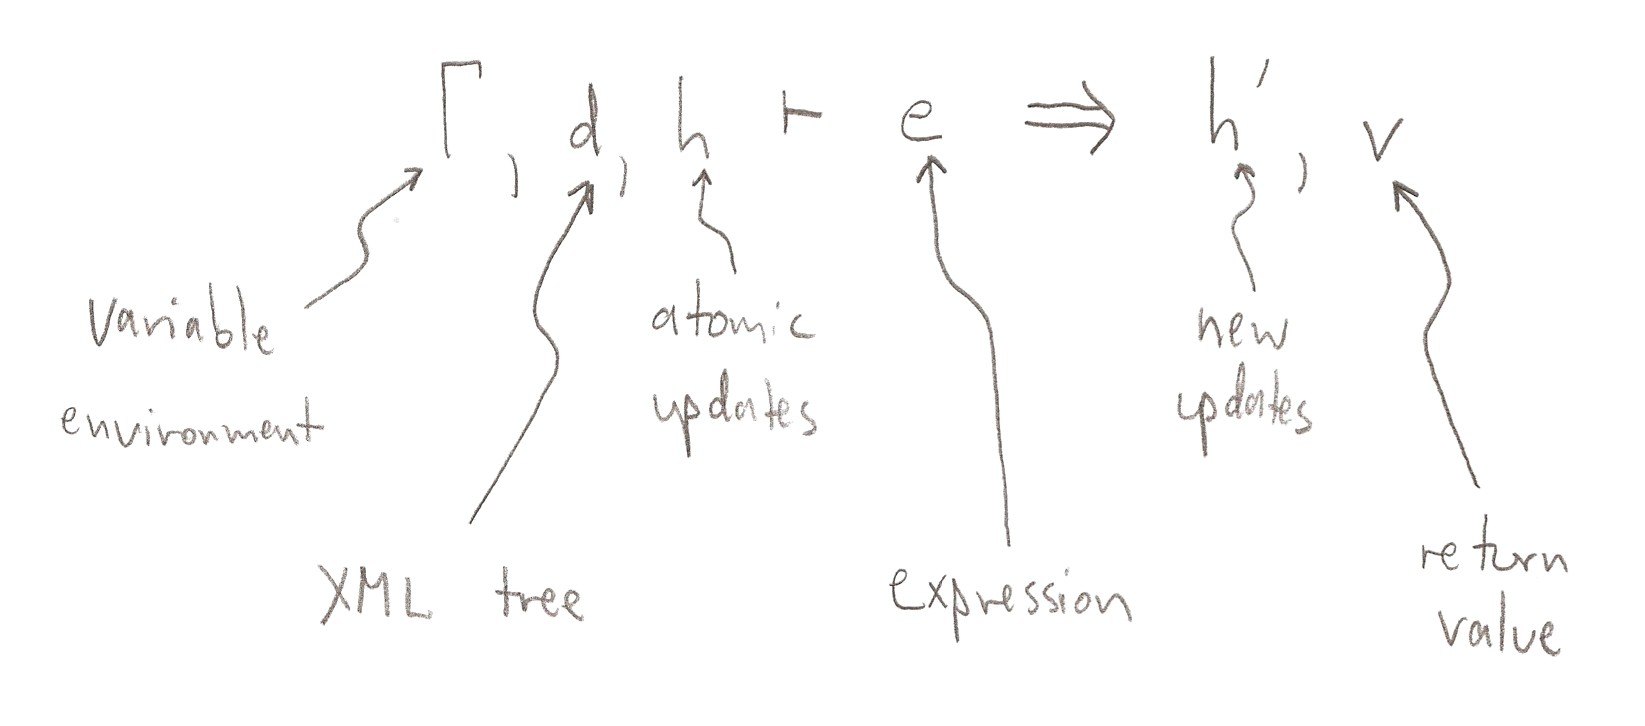
\includegraphics[width=\linewidth]{cjudgment.jpg}
    \end{center}
\end{frame}

\begin{frame}
    \frametitle{Sample Judgment Rules}
    \infrule
        {\Gamma;d;h_0 \vdash e_1 \Rightarrow h_1;v_1 \\
         \Gamma;d;h_0,h_1 \vdash e_2 \Rightarrow h_2;v_2}
        {\Gamma;d;h_0 \vdash e_1,e_2 \Rightarrow h_1,h_2;v_1,v_2}
    \vfil
    \infrule
        {\Gamma;d;h \vdash e \Rightarrow h';\ell_1,\ldots,\ell_n}
        {\Gamma;d;h \vdash \edelete e \Rightarrow
        h',\mbox{delete}(\ell_1),\ldots,\mbox{delete}(\ell_n);\langle\rangle}
\end{frame}

\begin{frame}
    \frametitle{Syntax}
    \begin{align*}
        e ::={}
            & x \mid e/A::T \mid e,e \mid \efor x \ein e \ereturn e \mid \\
            & e = e \mid \eif e \ethen e \eelse e \mid \eelement \loc e e \mid \\
            & \edelete e \mid \einsert e \einto e \mid \elet x := e \ein e \\
        A ::={} & \echild \mid \edescendant \mid \eparent \mid \eancestor \\
        T ::={} & \etext \mid \enode \mid q \mid *
    \end{align*}
\end{frame}

\begin{frame}
    \frametitle{Problem Statement}
    \begin{itemize}
        \item Alice sends update $e_A$
        \item Bob sends update $e_B$
        \item So, evaluating $e_A,e_B$
        \item But $e_B,e_A$ looks faster
        \item Is it safe?
    \end{itemize}
\end{frame}

\begin{frame}
    \frametitle{Examples}
    \begin{tabular}{ll}
        $e_A$ & $e_B$ \\
        \hline
        \edelete $doc$/wines/california & \efor $x$\ein $doc$//country \\
        &\ \ \ereturn $x$//name \\
        \\
        \edelete $doc$/wines/california & \efor $x$\ein $doc$/country \\
        &\ \ \ereturn \einsert \{\textless new/\textgreater\}\einto $x$ \\
        \\
        \efor $x$\ein $doc$/country & \efor $x$\ein $doc$//country \\
        \ \ \ereturn \edelete $x$/city &\ \ \ereturn $x$//name
    \end{tabular}
\end{frame}

\begin{frame}
    \frametitle{Main Idea}
    \begin{itemize}
        \item Keep track of \emph{paths} that are accessed and updated
        \item Commuting is safe when writes are disjoint from accesses
        \item Static analysis -- so overestimate
        \item $\Delta \vdash e \Rightarrow r;a;u$
    \end{itemize}
\end{frame}

\newcommand{\prefix}{\ensuremath{\mathit{pref}}}
\begin{frame}
    \frametitle{Paths}
    \[p ::= \varepsilon \mid \loc \mid p|p \mid p/A::T\]
    \vpause
    \begin{align*}
        \prefix(\varepsilon) &= \varepsilon \\
        \prefix(\loc) &= \varepsilon \\
        \prefix(p|q) &= \prefix(p)|\prefix(q) \\
        \prefix(p/a::t) &= p
    \end{align*}
\end{frame}

\newcounter{rulepart}
\newcommand{\ruletitle}[1]{\addtocounter{rulepart}{1}\frametitle{Static
Analysis Rules, Part \arabic{rulepart}: #1}}
\begin{frame}
    \ruletitle{Easy Rules}
    \infrule
        {(x \mapsto p) \in \Delta}
        {\Delta \vdash x \Rightarrow p;\varepsilon;\varepsilon}
    \vpause
    \infrule
        {\Delta \vdash e \Rightarrow p_r;p_a;p_u \\
         \Delta \vdash e' \Rightarrow p_r';p_a';p_u'}
        {\Delta \vdash e,e' \Rightarrow p_r|p_r';p_a|p_a';p_u|p_u'}
    \vpause
    Also easy: \textbf{element}, \textbf{let}, and axis selection
\end{frame}

\begin{frame}
    \ruletitle{For}
    \infrule
        {\Delta \vdash e \Rightarrow p_r;p_a;p_u \\
         \Delta,x \mapsto p_r \vdash e' \Rightarrow p_r';p_a';p_u'}
        {\Delta \vdash \efor x \ein e \ereturn e' \Rightarrow
        p_r';p_a|p_a';p_u|p_u'}
\end{frame}

\begin{frame}
    \ruletitle{If}
    \infrule
        {\Delta \vdash e \Rightarrow r;a;u \\
         \Delta \vdash e_t \Rightarrow r_t;a_t;u_t \\
         \Delta \vdash e_f \Rightarrow r_f;a_f;u_f}
        {\Delta \vdash \eif e \ethen e_t \eelse e_f \Rightarrow
        r|r_t|r_f;a|a_t|a_f;u|u_t|u_f}
\end{frame}

\begin{frame}
    \frametitle{Insert and Delete}
    \infrule
        {\Delta \vdash e \Rightarrow p_r;p_a;p_u}
        {\Delta \vdash \edelete e \Rightarrow
         \varepsilon;p_a;p_u|p_r|p_r/\edescendant::*}
    \vpause
    \infrule
        {\Delta \vdash e \Rightarrow p_r;p_a;p_u \\
         \Delta \vdash e' \Rightarrow p_r';p_a';p_u'}
        {\Delta \vdash \einsert e \einto e' \Rightarrow \\
         \varepsilon;p_a|p_a'|\prefix^*(p_r/\edescendant::*);p_u|p_u'|p_r'|p_r'/\edescendant::*}
\end{frame}

\begin{frame}
    \frametitle{Safe Commuting}
    If we have
    \[\Delta \vdash e \Rightarrow r;a;u\]
    \[\Delta \vdash e' \Rightarrow r';a';u'\]
    Then it's safe to commute $e$ and $e'$ when
    \[u\cap(a' \mid u')=u'\cap(a \mid u)=\emptyset\]
\end{frame}

% TODO: Path persistence in the face of deletion -- another reason it's hard

\begin{frame}
    \frametitle{Time For Questions!}
    Please, ask me more about
    \begin{itemize}
        \item Laying the groundwork for formalizing revision control systems' behavior
        \item Computing tree diffs
        \item Re-ordering database queries
    \end{itemize}
\end{frame}

\end{document}
